\section{Introduction}
\label{sec:intro}

With increasingly large deep learning models, hardware constraints often limit the feasible batch size that can fit within the memory (VRAM) of even the most powerful GPUs. Consequently, machine learning practitioners must distribute the training across hundreds or thousands of GPUs using Distributed Data Parallelism (DDP), Distributed Model Parallelism (DMP), or a combination of both \cite{li2020pytorch,dean2012large,shoeybi2019megatron,you2020large,hoffmann2022training}. As a result, the traditional minibatch in stochastic gradient descent (SGD) has been replaced with microbatches and macrobatches \cite{Piao_2023}. A microbatch is defined as the samples processed by a single forward and backward pass to produce a microbatch gradient, often called a micro-gradient. Microbatches are typically produced on a per GPU basis and then shared across all of the other GPUs to calculate the macrobatch. A macrobatch is the union of all microbatches. Each micro-gradient is summed and then normalized to compute the macro-gradient, which is then used to update the model. In practice, the microbatch size is chosen to maximize the VRAM utilization on a single GPU or computation node. During the aggregation of micro-gradients, practitioners leverage the Ring-AllReduce algorithm \cite{baidu2017ringallreduce} to efficiently aggregate micro-gradients across all computation nodes. Ring-AllReduce relies on sequential summation and normalization to ensure synchronization of gradient values across all nodes without each node needing to retain multiple micro-gradient copies in memory. Once all gradients from the macrobatch have been aggregated a parameter update is performed and the process is repeated.

\begin{figure*}[t!]
  \centering
  \begin{subfigure}{0.495\linewidth}
    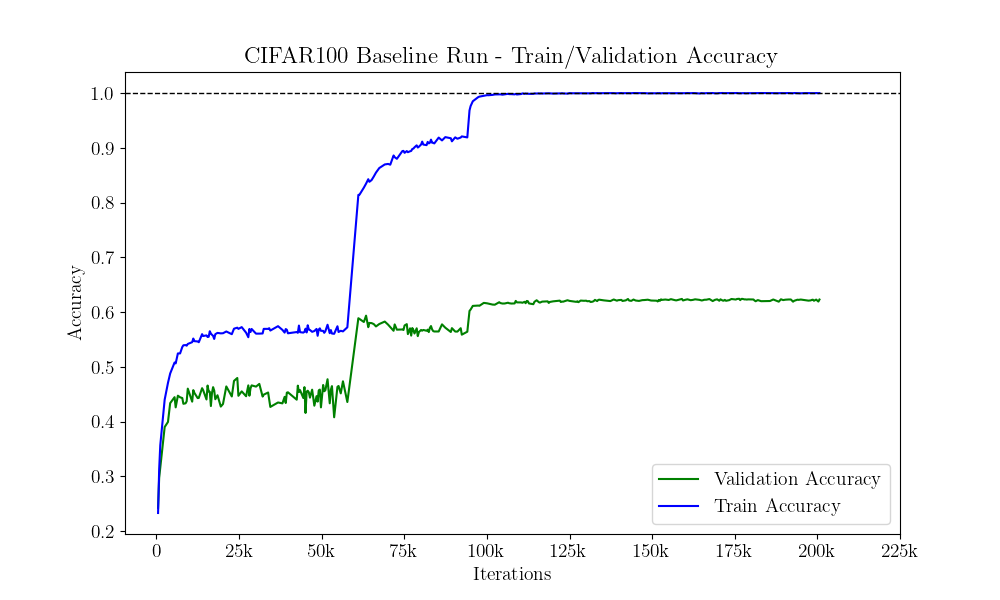
\includegraphics[width=\linewidth,  trim=0 0 0 17mm, clip]{figures/figure_1_1_Baseline_Run_CIFAR100.png}
    \caption{Train and validation accuracy over training on CIFAR-100}
    \label{fig:trainingval_cifar100}
  \end{subfigure}
  \hfill
  \begin{subfigure}{0.495\linewidth}
    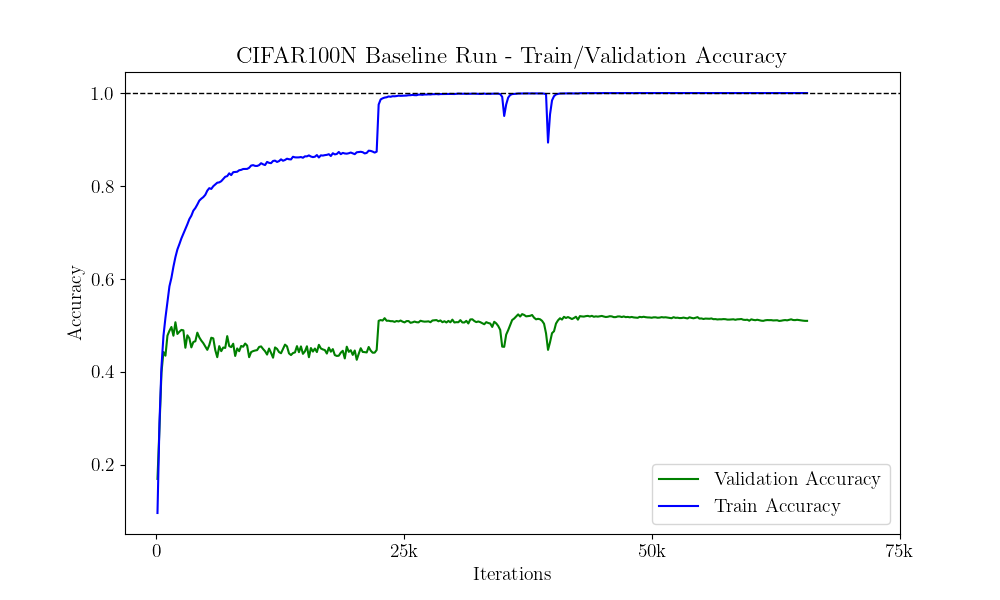
\includegraphics[width=\linewidth,  trim=0 0 0 17mm, clip]{figures/figure_1_2_Baseline_Run_CIFAR100N.png}
    \caption{Train and validation accuracy over training on CIFAR-100N-Fine}
    \label{fig:trainingval_cifar100n}
  \end{subfigure} \\
  \begin{subfigure}{0.495\linewidth}
    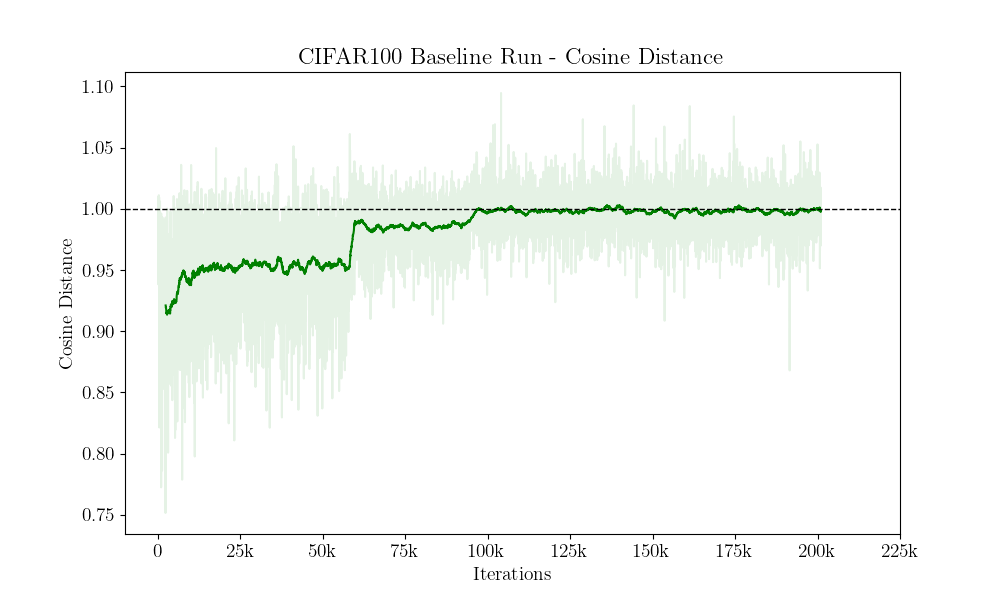
\includegraphics[width=\linewidth,  trim=0 0 0 17mm, clip]{figures/figure_1_3_Baseline_Run_CIFAR100_cosine_distance.png}
    \caption{Cosine distance over training on CIFAR-100}
    \label{fig:cosdist_cifar100}
  \end{subfigure}
  \hfill
  \begin{subfigure}{0.495\linewidth}
    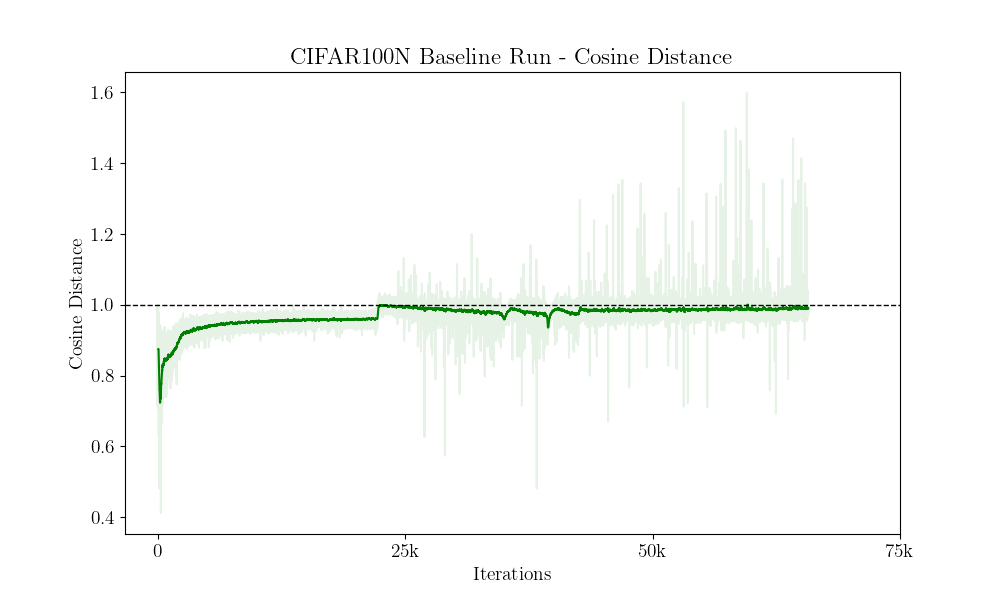
\includegraphics[width=\linewidth,  trim=0 0 0 17mm, clip]{figures/figure_1_4_Baseline_Run_CIFAR100N_cosine_distance.png}
    \caption{Cosine distance over training on CIFAR-100N-Fine}
    \label{fig:costdist_cifar100n}
  \end{subfigure}
  \caption{We train a ResNet18 on CIFAR-100 (left) and CIFAR-100N-Fine (right). We show train and validation accuracy  over iterations (top). The rolling average of cosine distances is shown in dark green and the raw cosine distances during training in light green (bottom). In late stages of training in all runs, as training accuracy plateaus, the cosine distance between micro-gradients approaches 1 with many micro-gradients diverging even further up to 1.1 for CIFAR-100 and 1.6 for CIFAR-100N-Fine. }
  \label{fig:val_cosd_cifar}
\end{figure*}

However, there is an underexplored question: is averaging all micro-gradients the best thing to do all of the time? Furthermore, are micro-gradients ever orthogonal or, worse, negatively correlated with each other during training? If so, what does this imply? This has been recently explored in the context of reinforcement learning for both multi-constraint  \cite{yao2023gradientshapingmulticonstraintsafe} and multi-task optimization \cite{yu2020gradientsurgerymultitasklearning} where gradients with respect to specific constraints or tasks are compared using cosine distance and update a projected component of the conflicting gradient onto the update direction or skip the gradient update altogether if the direction violates constraints. However, this has yet to be developed as a general optimization procedure, specifically in the context of distributed training. The first question we explore is what happens during typical training. Are the micro-gradients always correlated or are they orthogonal or divergent? To measure this, we compute the cosine distance between micro-gradients before averaging them over the course of training ResNet18 \cite{he2016deep} on both CIFAR-100 \cite{krizhevsky2009learning} and CIFAR-100N-Fine \cite{wei2022learning}. The cosine distance $D_c(\mathbf{x},\mathbf{y}) \in [0, 2]$ between two vectors $\mathbf{x}$ and $\mathbf{y}$ is used as a measure of divergence between the vectors. A cosine distance of 0 means two vectors are perfectly correlated, a cosine distance of 1 means they are orthogonal, and a cosine distance of 2 means they perfectly negatively correlated (pointed in the opposite directions). We find that during training micro-gradients are often orthogonal or negatively correlated with each other resulting in cosine distances close to or above 1 especially in late stages of training, as shown in \Cref{fig:cosdist_cifar100} and \Cref{fig:costdist_cifar100n}. The observation that micro-gradients are significantly misaligned, to the point of orthogonality or beyond, suggests that each microbatch offers a meaningfully different approximation of the true loss surface. This indicates that the optimization procedure should be cautious of stepping with these gradients as there is no consensus on which direction to take. This can be intuitively visualized in two dimensions as seen in \Cref{fig:micrograd_visual}.

\begin{figure}[ht!]
  \centering
  \begin{subfigure}{0.495\linewidth}
    \begin{tikzpicture}
        % Draw x and y coordinate axes
        \draw[->] (-2, 0) -- (2, 0) node[right] {};
        \draw[->] (0, -2) -- (0, 2) node[above] {};
    
        % Draw arrows at specified angles
        
        \foreach \angle in {260, 295, 335} { % {70, 205, 295}
            % Draw arrows at specified angles with labels
            \draw[->, thick, >=stealth] (0, 0) -- ({2*cos(\angle)}, {2*sin(\angle)})
                node[shift={(0.2,0.2)}, anchor=south] {};
        }
    \end{tikzpicture}
    \caption{Low cosine distance, $<1$}
    \label{fig:micrograd_aligned}
  \end{subfigure}
  \hfill
  \begin{subfigure}{0.495\linewidth}
    \begin{tikzpicture}
        % Draw x and y coordinate axes
        \draw[->] (-2, 0) -- (2, 0) node[right] {};
        \draw[->] (0, -2) -- (0, 2) node[above] {};
    
        % Draw arrows at specified angles
        
        \foreach \angle in {70, 205, 305} {
            % Draw arrows at specified angles with labels
            \draw[->, thick, >=stealth] (0, 0) -- ({2*cos(\angle)}, {2*sin(\angle)})
                node[shift={(0.2,0.2)}, anchor=south] {};
        }
    \end{tikzpicture}
    \caption{High-cosine distance, $\geq 1$}
    \label{fig:micrograd_misaligned}
  \end{subfigure}
  \caption{Visualization of cosine distance between micro-gradient batches in 2D. Aligned gradients have low cosine distance (left), while orthogonal or negatively correlated gradients have high cosine distance (right).}
  \label{fig:micrograd_visual}
\end{figure}

When training image classification models, we find that this pattern exists across all tested model sizes and datasets. Micro-gradients exhibit a high cosine distance (close to or above 1) during both very early and late stages of training. This was observed in both smaller models such as ResNet18 (11 million parameters) on CIFAR-100, as shown in \Cref{fig:cosdist_cifar100} and \Cref{fig:costdist_cifar100n}, and  larger models such as ViT-L/16 (300 million parameters) \cite{dosovitskiy2021an} trained on ImageNet (ILSVRC12) \cite{5206848}, as shown in \Cref{fig:baseline_vit_run}. Large cosine distances in both early and late stages of training can be explained by the information bottleneck principle \cite{tishby2015deep}. In early stages of training, the randomly initialized weights lack well-formed kernels that are able to produce activations with high mutual information with the training set, and each microbatch may easily disagree on where in the model to place each of these kernels or features. In later stages of training, when these kernels or features are well-formed and training accuracy nears 100\%, micro-gradient misalignment implies that at least one of the micro-gradient directions is a step into memorizing each individual microbatch, instead of a step into further generalizing on the validation set. In either case, we show skipping these steps results in more stable training and less overfitting which is the core idea of this paper.

The conventional way to train deep models in a stable way has been to increase batch size to average out noise-induced variances up to the point of diminishing returns where larger batch sizes beyond some critical point result in a reduction in generalization \cite{keskar2016large,arpit2017closer,mccandlish2018empirical}, with increased computational cost and risk of memorizing noisy labels. We see that as the microbatch size increases the micro-gradients across 2 microbatches become increasingly correlated, as shown in \Cref{fig:baseline_cifar100_batchsize}. This would be true even in the presence of noise in the dataset as per the law of large numbers. When taken to the limit of setting the microbatch size equal to the entire training set, the cosine distance clearly would approach 0. This implies that there is an optimal batch size for every training run. This was explored by \citeauthor{mccandlish2018empirical} where beyond this critical point, called the critical batch size, increasing macro-batch size further only increases computational cost without significant training benefit. However, these critical batch sizes are still often quite large. For example, the current state-of-the-art image classification model uses a batch size of 4096 which requires 8.2TB of VRAM in distributed training. What if we can achieve equal or better generalization at batch sizes far beneath \citeauthor{mccandlish2018empirical}'s critical batch size by leveraging our knowledge of divergent micro-gradients? 

\begin{figure}[ht]
    \centering
    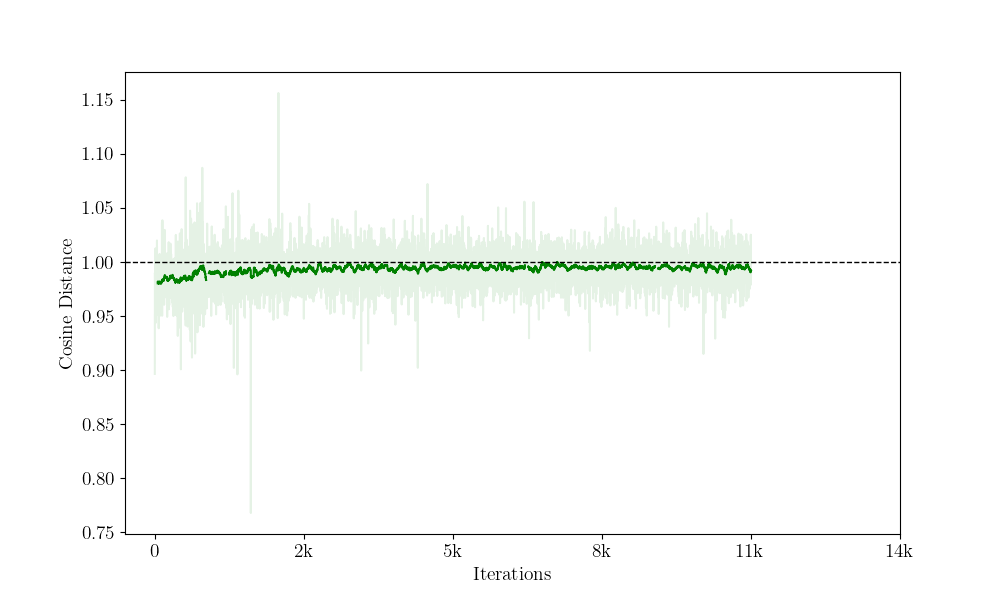
\includegraphics[width=0.975\linewidth]{figures/figure_1_5_Baseline_Run_ImageNet_ViT_L_Cosine_Distance.png}
    \caption{Cosine distances between micro-gradients during the later stages of a baseline ViT-L/16 run on ILSVRC12}
    \label{fig:baseline_vit_run}
\end{figure}

\begin{figure}[ht]
    \centering
    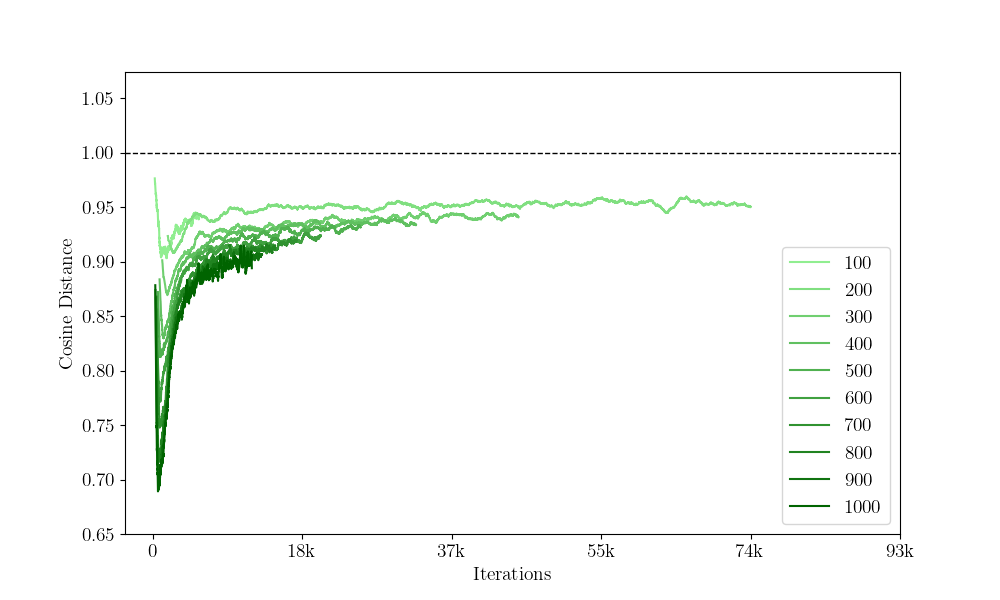
\includegraphics[width=0.975\linewidth]{figures/figure_2_Baseline_Run_CIFAR100_over_Batch_Size_3.png}
    \caption{Rolling average of cosine distances between micro-gradients during 10 baseline runs on CIFAR-100 varying batch sizes from 100 to 1000. As the microbatch size increases, the micro-gradients become more and more correlated throughout training.}
    \label{fig:baseline_cifar100_batchsize}
\end{figure}

This paper presents a solution that achieves equal to or higher generalization with much smaller batch sizes by calculating the cosine distances between micro-gradients and filtering out those that have high cosine distance from each other during aggregation, prior to performing the gradient update. This approach, called Gradient Agreement Filtering (GAF), leads to fewer accepted micro-gradients which significantly increases generalization and robustness, especially in the presence of noisy data. In \Cref{sec:prior_work} we discuss relevant related works. Next in \Cref{sec:methods} we introduce the core concepts and algorithmic implementation. Finally, in \Cref{sec:experiments} we demonstrate the efficacy of GAF on training ResNet18 and ResNet34 image classifiers on CIFAR-100 and CIFAR-100N-Fine, datasets respectively, where we find that adding GAF improves validation accuracy from 0.2\% to 18\%, with only a batch size of 200 (a microbatch size of 100 and a macrobatch size of 2). This outperforms the non-GAF baseline runs over all batch sizes, up to and including batches as large as 1100. We also show that as microbatch size increases in GAF-based training, this improvement decreases as the signal washes out. This suggests smaller micro-gradients with GAF are better for generalization, robustness to noisy labels, and compute.

% aggregating reduces memorization of noise,  and can yield the same or even improved accuracy, particularly in the presence of noise in our train set, with an order of magnitude less compute. As shown in Figure~\Cref{fig:cifar100_over_noise_results}, GAF can improve validation accuracy by more than 18\%. \\

\section{Previous Works}
\label{sec:prior_work}

Gradient descent has been fundamental to machine learning since the 1950s. Initial works introduced the basic iterative framework for gradient descent and soon led to the development of stochastic gradient descent (SGD)~\cite{robbins1951sgd}, which computes gradients on small, random subsets of data rather than the entire dataset, enabling efficient optimization in high-dimensional settings. Building upon this foundation, researchers have developed various enhancements to SGD, including \textit{momentum}~\cite{polyak1964some}, which introduces a velocity term to accelerate convergence in regions with low curvature, and \textit{Adam}~\cite{kingma2014adam}, which combines momentum with adaptive learning rates to better handle sparse gradients and noisy data. A recent refinement is, \textit{AdamW}~\cite{loshchilov2017decoupled}, decouples weight decay from the gradient update process, yielding better generalization properties by stabilizing the learning dynamics. In recent years, the deep learning community has produced a substantial body of research that addresses the practical challenges of gradient-based optimization.

% \subsection{Distributed and Parallel Training}

To handle the immense computational demands of training large models, researchers have explored various distributed and parallel training frameworks based on the concepts of data and model parallelism. These approaches enable practitioners to scale training across multiple GPUs or compute nodes, facilitating larger batch sizes and reducing the time required for model convergence. Techniques like \textit{Ring-AllReduce}~\cite{baidu2017ringallreduce} allow for efficient gradient aggregation across GPUs, minimizing communication overhead, and memory, enabling synchronous training on high-performance systems. Additionally, asynchronous gradient sharing strategies and parameter servers~\cite{dean2012large} have been proposed to further enhance scalability, though come at the cost of potential staleness in parameter updates.

% \subsection{Robust and Adaptive Optimizers}

Adaptive optimization algorithms, including \textit{RMSProp}~\cite{tieleman2012lecture} and \textit{Adam}~\cite{kingma2014adam}, address the limitations of standard SGD by dynamically adjusting learning rates based on historical gradient information. These methods have proven especially useful in handling noisy or sparse gradients, which are common in large-scale deep learning models. Recent advancements, such as layer-wise adaptive moments (\textit{LAMB})~\cite{you2020large} and \textit{AdaBelief}~\cite{zhuang2020adabelief} focus on improving generalization by adapting learning rates according to layer-specific characteristics or reducing reliance on gradient magnitudes to mitigate training instability.

% \subsection{Generalization and Overfitting Control}

A challenge in deep learning is the balance between fitting the training data well while simultaneously avoiding overfitting and memorizing train noise. Researchers have proposed various strategies to control overfitting, such as data augmentation, dropout~\cite{srivastava2014dropout}, and early stopping~\cite{prechelt1998early}. Recent work on sharpness-aware minimization (\textit{SAM})~\cite{foret2020sharpness} explicitly targets solutions within flatter regions of the loss landscape to promote generalization, which has shown significant promise across various deep learning benchmarks.

% \subsection{Robustness to Noisy Labels in our Training Set}

Training deep models in the presence of noisy labels is a challenging problem, as noise can lead to memorization of incorrect labels and hinder generalization. Several methods have been proposed to address label noise, including learning from noisy labels~\cite{li2020learning}, co-teaching~\cite{han2018coteaching}, and learning to learn from noisy labels~\cite{ren2018learning}. These methods often rely on a dual-network architecture, where one network acts as a teacher or peer model to guide the student model in selectively learning from clean samples. This approach, however, is computationally expensive as it requires training two instances of the same model in parallel, which scales poorly for large models and datasets. More recent approaches, such as self-supervised over-parametrization (\textit{SOP})~\cite{liu2022self}, utilize an expectation-maximization technique to address label noise by leveraging over-parameterized models, though this method also incurs substantial additional computational costs. \textit{DivideMix}~\cite{li2020dividemix} and \textit{ProMix}~\cite{xiao2023promix} introduce techniques for probabilistic mixing of samples, aiming to filter noisy samples during training, but they still rely on computationally intensive procedures to maintain robust performance. The sample priors* framework~\cite{chen2023sample} employs sample reweighting based on prior distributions to discount noisy labels, but it similarly requires additional model components that limit its scalability.

% \subsection{Generalized Learning and Batch Size Scaling}

The choice of batch size plays a crucial role in the trade-off between training stability and generalization. Studies by~\cite{mccandlish2018empirical} have shown that batch sizes up to a certain critical threshold stabilize model performance, whereas larger batch sizes tend to degrade generalization due to reduced gradient noise. Further studies have proposed batch-size scaling rules and scaling laws for adapting learning rate with batch size to optimize training efficiency and convergence~\cite{goyal2018accuratelargeminibatchsgd}.

% \subsection{Efficient Gradient Aggregation and Filtering}

Recent research has also focused on optimizing the gradient aggregation process itself. Techniques like gradient clipping~\cite{pascanu2013difficultytrainingrecurrentneural} help stabilize training by capping the norm of gradients, particularly in recurrent neural networks where gradient explosion is common. Further, gradient noise injection~\cite{neelakantan2015addinggradientnoiseimproves} has been explored as a means to escape sharp local minima and prevent overfitting. Our work builds on this line of inquiry by introducing gradient agreement filtering, a novel approach to dynamically filter micro-gradients based on cosine distance, allowing us to improve computational efficiency by reducing batch sizes while still maintaining training stability by excluding high-disagreement gradients in each macrobatch.
